\documentclass[twoside]{book}

% Packages required by doxygen
\usepackage{fixltx2e}
\usepackage{calc}
\usepackage{doxygen}
\usepackage[export]{adjustbox} % also loads graphicx
\usepackage{graphicx}
\usepackage[utf8]{inputenc}
\usepackage{makeidx}
\usepackage{multicol}
\usepackage{multirow}
\PassOptionsToPackage{warn}{textcomp}
\usepackage{textcomp}
\usepackage[nointegrals]{wasysym}
\usepackage[table]{xcolor}

% Font selection
\usepackage[T1]{fontenc}
\usepackage[scaled=.90]{helvet}
\usepackage{courier}
\usepackage{amssymb}
\usepackage{sectsty}
\renewcommand{\familydefault}{\sfdefault}
\allsectionsfont{%
  \fontseries{bc}\selectfont%
  \color{darkgray}%
}
\renewcommand{\DoxyLabelFont}{%
  \fontseries{bc}\selectfont%
  \color{darkgray}%
}
\newcommand{\+}{\discretionary{\mbox{\scriptsize$\hookleftarrow$}}{}{}}

% Page & text layout
\usepackage{geometry}
\geometry{%
  a4paper,%
  top=2.5cm,%
  bottom=2.5cm,%
  left=2.5cm,%
  right=2.5cm%
}
\tolerance=750
\hfuzz=15pt
\hbadness=750
\setlength{\emergencystretch}{15pt}
\setlength{\parindent}{0cm}
\setlength{\parskip}{3ex plus 2ex minus 2ex}
\makeatletter
\renewcommand{\paragraph}{%
  \@startsection{paragraph}{4}{0ex}{-1.0ex}{1.0ex}{%
    \normalfont\normalsize\bfseries\SS@parafont%
  }%
}
\renewcommand{\subparagraph}{%
  \@startsection{subparagraph}{5}{0ex}{-1.0ex}{1.0ex}{%
    \normalfont\normalsize\bfseries\SS@subparafont%
  }%
}
\makeatother

% Headers & footers
\usepackage{fancyhdr}
\pagestyle{fancyplain}
\fancyhead[LE]{\fancyplain{}{\bfseries\thepage}}
\fancyhead[CE]{\fancyplain{}{}}
\fancyhead[RE]{\fancyplain{}{\bfseries\leftmark}}
\fancyhead[LO]{\fancyplain{}{\bfseries\rightmark}}
\fancyhead[CO]{\fancyplain{}{}}
\fancyhead[RO]{\fancyplain{}{\bfseries\thepage}}
\fancyfoot[LE]{\fancyplain{}{}}
\fancyfoot[CE]{\fancyplain{}{}}
\fancyfoot[RE]{\fancyplain{}{\bfseries\scriptsize Generated by Doxygen }}
\fancyfoot[LO]{\fancyplain{}{\bfseries\scriptsize Generated by Doxygen }}
\fancyfoot[CO]{\fancyplain{}{}}
\fancyfoot[RO]{\fancyplain{}{}}
\renewcommand{\footrulewidth}{0.4pt}
\renewcommand{\chaptermark}[1]{%
  \markboth{#1}{}%
}
\renewcommand{\sectionmark}[1]{%
  \markright{\thesection\ #1}%
}

% Indices & bibliography
\usepackage{natbib}
\usepackage[titles]{tocloft}
\setcounter{tocdepth}{3}
\setcounter{secnumdepth}{5}
\makeindex

% Hyperlinks (required, but should be loaded last)
\usepackage{ifpdf}
\ifpdf
  \usepackage[pdftex,pagebackref=true]{hyperref}
\else
  \usepackage[ps2pdf,pagebackref=true]{hyperref}
\fi
\hypersetup{%
  colorlinks=true,%
  linkcolor=blue,%
  citecolor=blue,%
  unicode%
}

% Custom commands
\newcommand{\clearemptydoublepage}{%
  \newpage{\pagestyle{empty}\cleardoublepage}%
}

\usepackage{caption}
\captionsetup{labelsep=space,justification=centering,font={bf},singlelinecheck=off,skip=4pt,position=top}

%===== C O N T E N T S =====

\begin{document}

% Titlepage & ToC
\hypersetup{pageanchor=false,
             bookmarksnumbered=true,
             pdfencoding=unicode
            }
\pagenumbering{roman}
\begin{titlepage}
\vspace*{7cm}
\begin{center}%
{\Large My Project }\\
\vspace*{1cm}
{\large Generated by Doxygen 1.8.11}\\
\end{center}
\end{titlepage}
\clearemptydoublepage
\tableofcontents
\clearemptydoublepage
\pagenumbering{arabic}
\hypersetup{pageanchor=true}

%--- Begin generated contents ---
\chapter{Class Index}
\section{Class List}
Here are the classes, structs, unions and interfaces with brief descriptions\+:\begin{DoxyCompactList}
\item\contentsline{section}{\hyperlink{structnode}{node} }{\pageref{structnode}}{}
\item\contentsline{section}{\hyperlink{structnode1}{node1} }{\pageref{structnode1}}{}
\item\contentsline{section}{\hyperlink{structnode__info}{node\+\_\+info} }{\pageref{structnode__info}}{}
\end{DoxyCompactList}

\chapter{File Index}
\section{File List}
Here is a list of all files with brief descriptions\+:\begin{DoxyCompactList}
\item\contentsline{section}{\hyperlink{Lab1_8c}{Lab1.\+c} }{\pageref{Lab1_8c}}{}
\end{DoxyCompactList}

\chapter{Class Documentation}
\hypertarget{classAlgebraicExpression}{}\section{Algebraic\+Expression Class Reference}
\label{classAlgebraicExpression}\index{Algebraic\+Expression@{Algebraic\+Expression}}


{\ttfamily \#include $<$Algebraic\+Expression.\+h$>$}



Collaboration diagram for Algebraic\+Expression\+:
\nopagebreak
\begin{figure}[H]
\begin{center}
\leavevmode
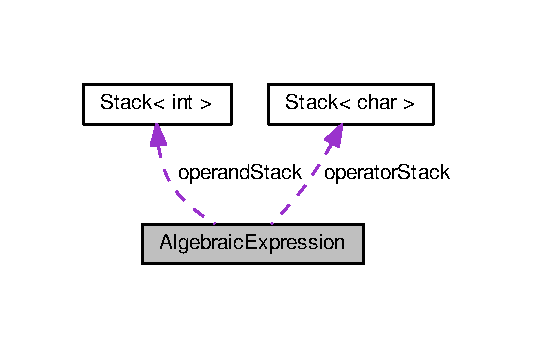
\includegraphics[width=257pt]{classAlgebraicExpression__coll__graph}
\end{center}
\end{figure}
\subsection*{Public Member Functions}
\begin{DoxyCompactItemize}
\item 
\hyperlink{classAlgebraicExpression_ae80b781e8b44002cdadf57fd4f092a8d}{Algebraic\+Expression} ()
\item 
\hyperlink{classAlgebraicExpression_aabfd3685b5e424afcf6fd0766820f953}{Algebraic\+Expression} (string s)
\item 
void \hyperlink{classAlgebraicExpression_ac0428ac1f1072f14e1391527baebd330}{evaluate\+Postfix} ()
\item 
void \hyperlink{classAlgebraicExpression_a0aeff15e3d0d529bd20a59f8d312a38d}{evaluate\+Infix} ()
\item 
int \hyperlink{classAlgebraicExpression_afcf555b573e6083a8395677bf056aef1}{get\+Result} ()
\item 
bool \hyperlink{classAlgebraicExpression_aa3c08af8a2b4d67c356f3cf69b2f6bc6}{valid} ()
\end{DoxyCompactItemize}
\subsection*{Private Member Functions}
\begin{DoxyCompactItemize}
\item 
bool \hyperlink{classAlgebraicExpression_a59e33cea19abab195b1c755347d07bf5}{precedence} (char op1, char op2)
\end{DoxyCompactItemize}
\subsection*{Private Attributes}
\begin{DoxyCompactItemize}
\item 
\hyperlink{classStack}{Stack}$<$ char $>$ \hyperlink{classAlgebraicExpression_a863ef1cc73b9b3b49c199f1564cbcc2e}{operator\+Stack}
\item 
\hyperlink{classStack}{Stack}$<$ int $>$ \hyperlink{classAlgebraicExpression_a8f0ee1ac59e782a546a7de47e507b391}{operand\+Stack}
\item 
int \hyperlink{classAlgebraicExpression_a13af7ae171ff8616e6ab013a9cee9d75}{result}
\item 
string \hyperlink{classAlgebraicExpression_ac9a5d8af4bd13370e7f2cb66b0f1daa2}{infix}
\item 
string \hyperlink{classAlgebraicExpression_a0c9827f84bf13c0f0f4a096e72462a44}{postfix}
\end{DoxyCompactItemize}
\subsection*{Friends}
\begin{DoxyCompactItemize}
\item 
istream \& \hyperlink{classAlgebraicExpression_af703364bc81e99767331bb9e915ef6ff}{operator$>$$>$} (istream \&ins, \hyperlink{classAlgebraicExpression}{Algebraic\+Expression} \&ae)
\end{DoxyCompactItemize}


\subsection{Constructor \& Destructor Documentation}
\index{Algebraic\+Expression@{Algebraic\+Expression}!Algebraic\+Expression@{Algebraic\+Expression}}
\index{Algebraic\+Expression@{Algebraic\+Expression}!Algebraic\+Expression@{Algebraic\+Expression}}
\subsubsection[{\texorpdfstring{Algebraic\+Expression()}{AlgebraicExpression()}}]{\setlength{\rightskip}{0pt plus 5cm}Algebraic\+Expression\+::\+Algebraic\+Expression (
\begin{DoxyParamCaption}
{}
\end{DoxyParamCaption}
)}\hypertarget{classAlgebraicExpression_ae80b781e8b44002cdadf57fd4f092a8d}{}\label{classAlgebraicExpression_ae80b781e8b44002cdadf57fd4f092a8d}

\begin{DoxyCode}
13 \{
14    \hyperlink{classAlgebraicExpression_a13af7ae171ff8616e6ab013a9cee9d75}{result} = 0;
15    \hyperlink{classAlgebraicExpression_ac9a5d8af4bd13370e7f2cb66b0f1daa2}{infix} = \textcolor{stringliteral}{""};
16    \hyperlink{classAlgebraicExpression_a0c9827f84bf13c0f0f4a096e72462a44}{postfix} = \textcolor{stringliteral}{""};
17 \}
\end{DoxyCode}
\index{Algebraic\+Expression@{Algebraic\+Expression}!Algebraic\+Expression@{Algebraic\+Expression}}
\index{Algebraic\+Expression@{Algebraic\+Expression}!Algebraic\+Expression@{Algebraic\+Expression}}
\subsubsection[{\texorpdfstring{Algebraic\+Expression(string s)}{AlgebraicExpression(string s)}}]{\setlength{\rightskip}{0pt plus 5cm}Algebraic\+Expression\+::\+Algebraic\+Expression (
\begin{DoxyParamCaption}
\item[{string}]{s}
\end{DoxyParamCaption}
)}\hypertarget{classAlgebraicExpression_aabfd3685b5e424afcf6fd0766820f953}{}\label{classAlgebraicExpression_aabfd3685b5e424afcf6fd0766820f953}

\begin{DoxyCode}
20 \{
21    \hyperlink{classAlgebraicExpression_a13af7ae171ff8616e6ab013a9cee9d75}{result} = 0;
22    \hyperlink{classAlgebraicExpression_ac9a5d8af4bd13370e7f2cb66b0f1daa2}{infix} = s;
23    \hyperlink{classAlgebraicExpression_a0c9827f84bf13c0f0f4a096e72462a44}{postfix} = \textcolor{stringliteral}{""};
24 \}
\end{DoxyCode}


\subsection{Member Function Documentation}
\index{Algebraic\+Expression@{Algebraic\+Expression}!evaluate\+Infix@{evaluate\+Infix}}
\index{evaluate\+Infix@{evaluate\+Infix}!Algebraic\+Expression@{Algebraic\+Expression}}
\subsubsection[{\texorpdfstring{evaluate\+Infix()}{evaluateInfix()}}]{\setlength{\rightskip}{0pt plus 5cm}void Algebraic\+Expression\+::evaluate\+Infix (
\begin{DoxyParamCaption}
{}
\end{DoxyParamCaption}
)}\hypertarget{classAlgebraicExpression_a0aeff15e3d0d529bd20a59f8d312a38d}{}\label{classAlgebraicExpression_a0aeff15e3d0d529bd20a59f8d312a38d}

\begin{DoxyCode}
75 \{
76    \textcolor{keywordtype}{char} c, op;
77    \textcolor{keywordtype}{int} i;
78    \textcolor{keywordflow}{if}(\hyperlink{classAlgebraicExpression_aa3c08af8a2b4d67c356f3cf69b2f6bc6}{valid}()) \textcolor{comment}{//only evaluates infix expression if equation is valid                                 
                                                                                                            }
79    \{
80       \textcolor{keywordflow}{for}(\textcolor{keywordtype}{int} k=0; k<\hyperlink{classAlgebraicExpression_ac9a5d8af4bd13370e7f2cb66b0f1daa2}{infix}.length(); k++) \textcolor{comment}{//loops through the infix expression                        
                                                                                                            }
81       \{
82          c = \hyperlink{classAlgebraicExpression_ac9a5d8af4bd13370e7f2cb66b0f1daa2}{infix}.at(k);
83          i = int(c) - int(\textcolor{charliteral}{'0'});
84          \textcolor{keywordflow}{if}(i >= 0 && i <= 9) \textcolor{comment}{//operand                                                                    
                                                                                                       }
85             \hyperlink{classAlgebraicExpression_a0c9827f84bf13c0f0f4a096e72462a44}{postfix} += c; \textcolor{comment}{//append operand to postfix string                                        
                                                                                                              }
86          \textcolor{keywordflow}{else} \textcolor{keywordflow}{if}(c == \textcolor{charliteral}{'('})
87             \hyperlink{classAlgebraicExpression_a863ef1cc73b9b3b49c199f1564cbcc2e}{operatorStack}.\hyperlink{classStack_a3553a0aa2c9640c5266e4d8790863e2e}{push}(c); \textcolor{comment}{//add opening parentheses to stack                     
                                                                                                                  
            }
88          \textcolor{keywordflow}{else} \textcolor{keywordflow}{if}(c == \textcolor{charliteral}{')'})
89          \{
90             op = \hyperlink{classAlgebraicExpression_a863ef1cc73b9b3b49c199f1564cbcc2e}{operatorStack}.\hyperlink{classStack_ad461f6de40c8672dbf743068f4515061}{top}();
91             \textcolor{keywordflow}{while}(op != \textcolor{charliteral}{'('}) \textcolor{comment}{//until closing opening parentheses is found                                  
                                                                                                       }
92             \{
93                \hyperlink{classAlgebraicExpression_a0c9827f84bf13c0f0f4a096e72462a44}{postfix} += op; \textcolor{comment}{//add operator to postfix string                                      
                                                                                                              }
94                op = \hyperlink{classAlgebraicExpression_a863ef1cc73b9b3b49c199f1564cbcc2e}{operatorStack}.\hyperlink{classStack_ad461f6de40c8672dbf743068f4515061}{top}(); \textcolor{comment}{//get next element from stack                     
                                                                                                                  
           }
95             \}
96          \}
97          \textcolor{keywordflow}{else} \textcolor{keywordflow}{if}(c == \textcolor{charliteral}{'+'}||c == \textcolor{charliteral}{'-'}||c == \textcolor{charliteral}{'*'}||c == \textcolor{charliteral}{'/'}) \textcolor{comment}{//operator                                        
                                                                                                       }
98          \{
99             \textcolor{keywordflow}{if}(!\hyperlink{classAlgebraicExpression_a863ef1cc73b9b3b49c199f1564cbcc2e}{operatorStack}.\hyperlink{classStack_ad0db0d9b249e871bb7504ed89a99d3a7}{isEmpty}())
100             \{
101                op = \hyperlink{classAlgebraicExpression_a863ef1cc73b9b3b49c199f1564cbcc2e}{operatorStack}.\hyperlink{classStack_adcb4774ac8aa94cbc19b461da9bdee3a}{peek}(); \textcolor{comment}{//look at top of stack, but don't access it     
                                                                                                                  
            }
102                \textcolor{keywordflow}{while}(!\hyperlink{classAlgebraicExpression_a863ef1cc73b9b3b49c199f1564cbcc2e}{operatorStack}.\hyperlink{classStack_ad0db0d9b249e871bb7504ed89a99d3a7}{isEmpty}() && op != \textcolor{charliteral}{'('} && 
      \hyperlink{classAlgebraicExpression_a59e33cea19abab195b1c755347d07bf5}{precedence}(op, c))
103                \{
104                   \hyperlink{classAlgebraicExpression_a0c9827f84bf13c0f0f4a096e72462a44}{postfix} += \hyperlink{classAlgebraicExpression_a863ef1cc73b9b3b49c199f1564cbcc2e}{operatorStack}.\hyperlink{classStack_ad461f6de40c8672dbf743068f4515061}{top}(); \textcolor{comment}{//add operator of greater
       precedence to postfix string                                                                                        
                  }
105                   \textcolor{keywordflow}{if}(!\hyperlink{classAlgebraicExpression_a863ef1cc73b9b3b49c199f1564cbcc2e}{operatorStack}.\hyperlink{classStack_ad0db0d9b249e871bb7504ed89a99d3a7}{isEmpty}())
106                      op = \hyperlink{classAlgebraicExpression_a863ef1cc73b9b3b49c199f1564cbcc2e}{operatorStack}.\hyperlink{classStack_adcb4774ac8aa94cbc19b461da9bdee3a}{peek}();
107                \}
108             \}
109             \hyperlink{classAlgebraicExpression_a863ef1cc73b9b3b49c199f1564cbcc2e}{operatorStack}.\hyperlink{classStack_a3553a0aa2c9640c5266e4d8790863e2e}{push}(c); \textcolor{comment}{//add original operator to stack                       
                                                                                                                  
            }
110          \}
111       \}
112       \textcolor{keywordflow}{while}(!\hyperlink{classAlgebraicExpression_a863ef1cc73b9b3b49c199f1564cbcc2e}{operatorStack}.\hyperlink{classStack_ad0db0d9b249e871bb7504ed89a99d3a7}{isEmpty}()) \textcolor{comment}{//any leftover operators still on stack should be
       added to postfix string                                                                                    
               }
113       \{
114          op = \hyperlink{classAlgebraicExpression_a863ef1cc73b9b3b49c199f1564cbcc2e}{operatorStack}.\hyperlink{classStack_ad461f6de40c8672dbf743068f4515061}{top}();
115          \hyperlink{classAlgebraicExpression_a0c9827f84bf13c0f0f4a096e72462a44}{postfix} += op;
116       \}
117    \}
118    \textcolor{keywordflow}{else} \textcolor{comment}{//if equation is invalid, an error will occur and the program will end                             
                                                                                                       }
119    \{
120       cerr << \textcolor{stringliteral}{"\(\backslash\)nError: expression is invalid "} << endl;
121       exit( 1 ); \textcolor{comment}{// terminate program;                                                                     
                                                                                                       }
122    \}
123 \}
\end{DoxyCode}


Here is the call graph for this function\+:
\nopagebreak
\begin{figure}[H]
\begin{center}
\leavevmode
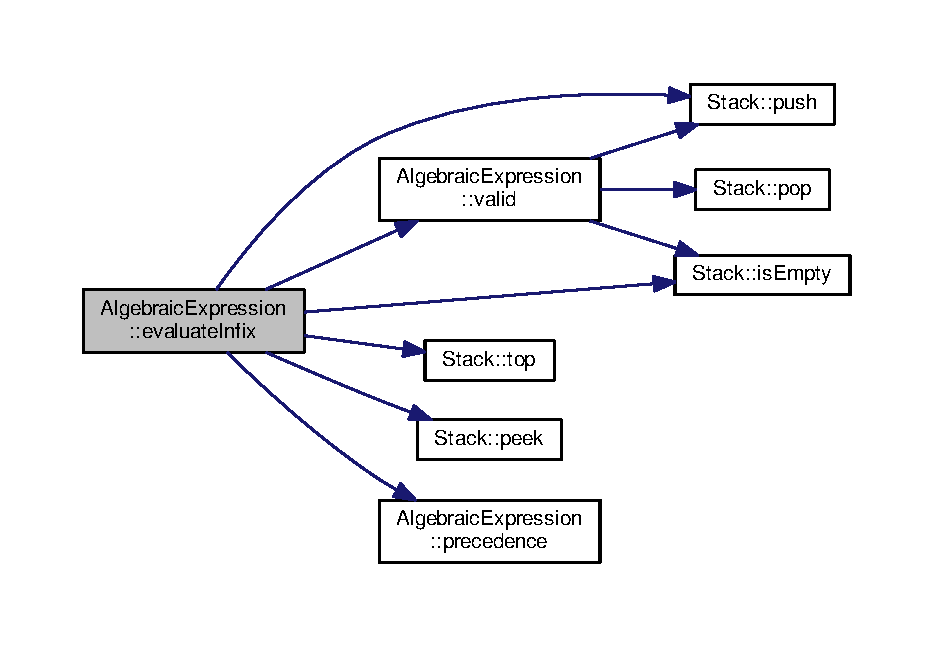
\includegraphics[width=350pt]{classAlgebraicExpression_a0aeff15e3d0d529bd20a59f8d312a38d_cgraph}
\end{center}
\end{figure}


\index{Algebraic\+Expression@{Algebraic\+Expression}!evaluate\+Postfix@{evaluate\+Postfix}}
\index{evaluate\+Postfix@{evaluate\+Postfix}!Algebraic\+Expression@{Algebraic\+Expression}}
\subsubsection[{\texorpdfstring{evaluate\+Postfix()}{evaluatePostfix()}}]{\setlength{\rightskip}{0pt plus 5cm}void Algebraic\+Expression\+::evaluate\+Postfix (
\begin{DoxyParamCaption}
{}
\end{DoxyParamCaption}
)}\hypertarget{classAlgebraicExpression_ac0428ac1f1072f14e1391527baebd330}{}\label{classAlgebraicExpression_ac0428ac1f1072f14e1391527baebd330}

\begin{DoxyCode}
27 \{
28    \textcolor{keywordtype}{char} c;
29    \textcolor{keywordtype}{int} i, op1, op2, r;
30    \textcolor{keywordflow}{if}(\hyperlink{classAlgebraicExpression_aa3c08af8a2b4d67c356f3cf69b2f6bc6}{valid}()) \textcolor{comment}{//if the equation is valid, the result will be calculated                              
                                                                                                            }
31    \{
32       \textcolor{keywordflow}{if}(\hyperlink{classAlgebraicExpression_a0c9827f84bf13c0f0f4a096e72462a44}{postfix}.length() >= 1) \textcolor{comment}{//makes sure that the equation has been converted to postfix
       expression                                                                                                     }
33       \{
34          \textcolor{keywordflow}{for}(\textcolor{keywordtype}{int} k=0; k<\hyperlink{classAlgebraicExpression_a0c9827f84bf13c0f0f4a096e72462a44}{postfix}.length(); k++) \textcolor{comment}{//loops through the entire postfix expression        
                                                                                                              }
35          \{
36             c = \hyperlink{classAlgebraicExpression_a0c9827f84bf13c0f0f4a096e72462a44}{postfix}.at(k);
37             i = int(c) - int(\textcolor{charliteral}{'0'});
38             \textcolor{keywordflow}{if}(i >= 0 && i <= 9) \textcolor{comment}{//operand                                                                 
                                                                                                       }
39                \hyperlink{classAlgebraicExpression_a8f0ee1ac59e782a546a7de47e507b391}{operandStack}.\hyperlink{classStack_a3553a0aa2c9640c5266e4d8790863e2e}{push}(i); \textcolor{comment}{//add operand to stack                                
                                                                                                                  
           }
40             \textcolor{keywordflow}{else} \textcolor{comment}{//operator                                                                                
                                                                                                       }
41             \{
42                op2 = \hyperlink{classAlgebraicExpression_a8f0ee1ac59e782a546a7de47e507b391}{operandStack}.\hyperlink{classStack_ad461f6de40c8672dbf743068f4515061}{top}(); \textcolor{comment}{//takes top two operands from stack for operation  
                                                                                                                  
          }
43                op1 = \hyperlink{classAlgebraicExpression_a8f0ee1ac59e782a546a7de47e507b391}{operandStack}.\hyperlink{classStack_ad461f6de40c8672dbf743068f4515061}{top}();
44                \textcolor{keywordflow}{if}(c == \textcolor{charliteral}{'+'})
45                   r = op1 + op2;
46                \textcolor{keywordflow}{else} \textcolor{keywordflow}{if}(c == \textcolor{charliteral}{'-'})
47                   r = op1 - op2;
48                \textcolor{keywordflow}{else} \textcolor{keywordflow}{if}(c == \textcolor{charliteral}{'*'})
49                   r = op1 * op2;
50                \textcolor{keywordflow}{else} \textcolor{keywordflow}{if}(c == \textcolor{charliteral}{'/'})
51                \{
52                   \textcolor{keywordflow}{if}(op2 != 0) \textcolor{comment}{//avoids division by 0                                                      
                                                                                                       }
53                      r = op1 / op2;
54                   \textcolor{keywordflow}{else} \textcolor{comment}{//if trying to divide by 0, error will occur and program will end                   
                                                                                                       }
55                   \{
56                      cerr << \textcolor{stringliteral}{"\(\backslash\)nError: cannot divide by 0 "} << endl;
57                      exit( 1 ); \textcolor{comment}{//terminate program;                                                       
                                                                                                       }
58                   \}
59                \}
60               \hyperlink{classAlgebraicExpression_a8f0ee1ac59e782a546a7de47e507b391}{operandStack}.\hyperlink{classStack_a3553a0aa2c9640c5266e4d8790863e2e}{push}(r); \textcolor{comment}{//returns the result of the operation to the stack     
                                                                                                                  
          }
61             \}
62          \}
63       \}
64       \textcolor{keywordflow}{if}(\hyperlink{classAlgebraicExpression_a8f0ee1ac59e782a546a7de47e507b391}{operandStack}.\hyperlink{classStack_a3091d98f798b1b3e69b644d5b778c428}{size}() == 1) \textcolor{comment}{//the only thing left on the stack is the result of the
       equation                                                                                                    
           }
65          \hyperlink{classAlgebraicExpression_a13af7ae171ff8616e6ab013a9cee9d75}{result} = \hyperlink{classAlgebraicExpression_a8f0ee1ac59e782a546a7de47e507b391}{operandStack}.\hyperlink{classStack_ad461f6de40c8672dbf743068f4515061}{top}();
66    \}
67    \textcolor{keywordflow}{else} \textcolor{comment}{//if equation is invalid, error will occur and program will end                                    
                                                                                                       }
68    \{
69       cerr << \textcolor{stringliteral}{"\(\backslash\)nError: expression is invalid "} << endl;
70       exit( 1 ); \textcolor{comment}{// terminate program;                                                                     
                                                                                                       }
71    \}
72 \}
\end{DoxyCode}


Here is the call graph for this function\+:
\nopagebreak
\begin{figure}[H]
\begin{center}
\leavevmode
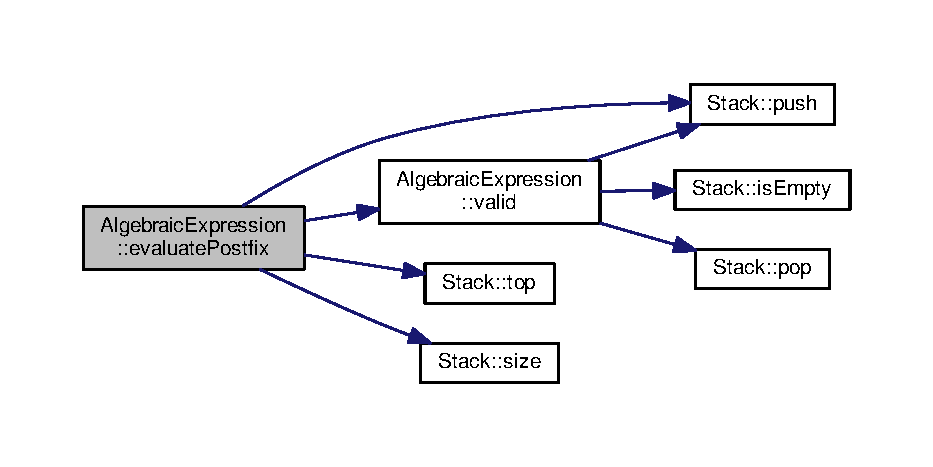
\includegraphics[width=350pt]{classAlgebraicExpression_ac0428ac1f1072f14e1391527baebd330_cgraph}
\end{center}
\end{figure}


\index{Algebraic\+Expression@{Algebraic\+Expression}!get\+Result@{get\+Result}}
\index{get\+Result@{get\+Result}!Algebraic\+Expression@{Algebraic\+Expression}}
\subsubsection[{\texorpdfstring{get\+Result()}{getResult()}}]{\setlength{\rightskip}{0pt plus 5cm}int Algebraic\+Expression\+::get\+Result (
\begin{DoxyParamCaption}
{}
\end{DoxyParamCaption}
)}\hypertarget{classAlgebraicExpression_afcf555b573e6083a8395677bf056aef1}{}\label{classAlgebraicExpression_afcf555b573e6083a8395677bf056aef1}

\begin{DoxyCode}
138 \{
139    \textcolor{keywordflow}{return} \hyperlink{classAlgebraicExpression_a13af7ae171ff8616e6ab013a9cee9d75}{result};
140 \}
\end{DoxyCode}
\index{Algebraic\+Expression@{Algebraic\+Expression}!precedence@{precedence}}
\index{precedence@{precedence}!Algebraic\+Expression@{Algebraic\+Expression}}
\subsubsection[{\texorpdfstring{precedence(char op1, char op2)}{precedence(char op1, char op2)}}]{\setlength{\rightskip}{0pt plus 5cm}bool Algebraic\+Expression\+::precedence (
\begin{DoxyParamCaption}
\item[{char}]{op1, }
\item[{char}]{op2}
\end{DoxyParamCaption}
)\hspace{0.3cm}{\ttfamily [private]}}\hypertarget{classAlgebraicExpression_a59e33cea19abab195b1c755347d07bf5}{}\label{classAlgebraicExpression_a59e33cea19abab195b1c755347d07bf5}

\begin{DoxyCode}
126 \{
127    \textcolor{comment}{//precendence if an op1 is greater than or equal to (in precendence) op2                                
                                                                                                       }
128    \textcolor{keywordtype}{bool} prec = \textcolor{keyword}{true}; \textcolor{comment}{//assume precedence                                                                   
                                                                                                       }
129    \textcolor{keywordflow}{if}(op1 == \textcolor{charliteral}{'+'} || op1 == \textcolor{charliteral}{'-'}) \textcolor{comment}{//if op1 is + or - and op2 is * or /, there is no precendence              
                                                                                                       }
130    \{
131          \textcolor{keywordflow}{if}(op2 == \textcolor{charliteral}{'*'} || op2 == \textcolor{charliteral}{'/'})
132             prec = \textcolor{keyword}{false};
133    \}
134    \textcolor{keywordflow}{return} prec;
135 \}
\end{DoxyCode}
\index{Algebraic\+Expression@{Algebraic\+Expression}!valid@{valid}}
\index{valid@{valid}!Algebraic\+Expression@{Algebraic\+Expression}}
\subsubsection[{\texorpdfstring{valid()}{valid()}}]{\setlength{\rightskip}{0pt plus 5cm}bool Algebraic\+Expression\+::valid (
\begin{DoxyParamCaption}
{}
\end{DoxyParamCaption}
)}\hypertarget{classAlgebraicExpression_aa3c08af8a2b4d67c356f3cf69b2f6bc6}{}\label{classAlgebraicExpression_aa3c08af8a2b4d67c356f3cf69b2f6bc6}

\begin{DoxyCode}
148 \{
149    \textcolor{keywordtype}{char} c, h;
150    \textcolor{keywordtype}{bool} \hyperlink{classAlgebraicExpression_aa3c08af8a2b4d67c356f3cf69b2f6bc6}{valid} = \textcolor{keyword}{true}; \textcolor{comment}{//assume valid                                                                  
                                                                                                            }
151    \hyperlink{classStack}{Stack<char>} paren, op;
152    \textcolor{keywordtype}{int} countOp=0, countInt=0, j, i;
153    \textcolor{keywordflow}{if}(\hyperlink{classAlgebraicExpression_ac9a5d8af4bd13370e7f2cb66b0f1daa2}{infix}.length() > 1)
154    \{
155       \textcolor{keywordflow}{for}(\textcolor{keywordtype}{int} k=0; k<\hyperlink{classAlgebraicExpression_ac9a5d8af4bd13370e7f2cb66b0f1daa2}{infix}.length(); k++) \textcolor{comment}{//loops though infix expression                             
                                                                                                            }
156       \{
157          c = \hyperlink{classAlgebraicExpression_ac9a5d8af4bd13370e7f2cb66b0f1daa2}{infix}.at(k);
158          i = int(c) - int(\textcolor{charliteral}{'0'});
159 
160          \textcolor{keywordflow}{if}(c == \textcolor{charliteral}{'('}) \textcolor{comment}{//checks if parentheses have pairs                                                   
                                                                                                       }
161             paren.\hyperlink{classStack_a3553a0aa2c9640c5266e4d8790863e2e}{push}(c);
162          \textcolor{keywordflow}{else} \textcolor{keywordflow}{if}(c == \textcolor{charliteral}{')'})
163          \{
164             \textcolor{keywordflow}{if}(!paren.\hyperlink{classStack_ad0db0d9b249e871bb7504ed89a99d3a7}{isEmpty}())
165                paren.\hyperlink{classStack_a2723aec5c7e2611b97fcffeb7709de33}{pop}();
166             \textcolor{keywordflow}{else}
167                valid = \textcolor{keyword}{false}; \textcolor{comment}{//no pair                                                                    
                                                                                                       }
168          \}
169          \textcolor{keywordflow}{else} \textcolor{keywordflow}{if}(c==\textcolor{charliteral}{'+'} || c==\textcolor{charliteral}{'*'} || c==\textcolor{charliteral}{'/'} || c==\textcolor{charliteral}{'-'}) \textcolor{comment}{//checks if each operator has two operands          
                                                                                                       }
170             op.\hyperlink{classStack_a3553a0aa2c9640c5266e4d8790863e2e}{push}(c);
171          \textcolor{keywordflow}{else} \textcolor{keywordflow}{if}(i>=0 && i<=9)
172          \{
173             \textcolor{keywordflow}{if}(!op.\hyperlink{classStack_ad0db0d9b249e871bb7504ed89a99d3a7}{isEmpty}())
174                op.\hyperlink{classStack_a2723aec5c7e2611b97fcffeb7709de33}{pop}();
175          \}
176       \}
177       \textcolor{keywordflow}{if}(!paren.\hyperlink{classStack_ad0db0d9b249e871bb7504ed89a99d3a7}{isEmpty}()) \textcolor{comment}{//no pair                                                                
                                                                                                              }
178          valid = \textcolor{keyword}{false};
179       \textcolor{keywordflow}{if}(!op.\hyperlink{classStack_ad0db0d9b249e871bb7504ed89a99d3a7}{isEmpty}()) \textcolor{comment}{//no two operands        }
180          valid = \textcolor{keyword}{false};
181    \}
182 
183    c = \hyperlink{classAlgebraicExpression_ac9a5d8af4bd13370e7f2cb66b0f1daa2}{infix}.at(0);
184    i = int(c) - int(\textcolor{charliteral}{'0'});
185    \textcolor{keywordflow}{if}(!(c == \textcolor{charliteral}{'('} || (i>=0 && i<=9))) \textcolor{comment}{//checks if the first element in the expression is a number or open
       parentheses                                                                                        }
186       valid = \textcolor{keyword}{false};
187 
188    \textcolor{keywordflow}{if}(\hyperlink{classAlgebraicExpression_ac9a5d8af4bd13370e7f2cb66b0f1daa2}{infix}.length() > 1)
189    \{
190       \textcolor{keywordflow}{for}(\textcolor{keywordtype}{int} k=0; k<\hyperlink{classAlgebraicExpression_ac9a5d8af4bd13370e7f2cb66b0f1daa2}{infix}.length()-1; k++)
191       \{
192          c = \hyperlink{classAlgebraicExpression_ac9a5d8af4bd13370e7f2cb66b0f1daa2}{infix}.at(k);
193          i = int(c) - int(\textcolor{charliteral}{'0'});
194          h = \hyperlink{classAlgebraicExpression_ac9a5d8af4bd13370e7f2cb66b0f1daa2}{infix}.at(k+1);
195          j = int(h) - int (\textcolor{charliteral}{'0'});
196          \textcolor{keywordflow}{if}(c == \textcolor{charliteral}{'('} && (h==\textcolor{charliteral}{'+'} || h==\textcolor{charliteral}{'-'} || h==\textcolor{charliteral}{'*'} || h==\textcolor{charliteral}{'/'})) \textcolor{comment}{// *(                                      
                                                                                                       }
197             valid = \textcolor{keyword}{false};
198          \textcolor{keywordflow}{if}(h == \textcolor{charliteral}{')'} && (c==\textcolor{charliteral}{'+'} || c==\textcolor{charliteral}{'-'} || c==\textcolor{charliteral}{'*'} || c==\textcolor{charliteral}{'/'})) \textcolor{comment}{// *)                                      
                                                                                                       }
199             valid = \textcolor{keyword}{false};
200          \textcolor{keywordflow}{if}(h == \textcolor{charliteral}{'('} && (i>=0 && i<=9)) \textcolor{comment}{// 9(                                                              
                                                                                                       }
201             valid = \textcolor{keyword}{false};
202          \textcolor{keywordflow}{if}(c == \textcolor{charliteral}{')'} && (j>=0 && j<=9)) \textcolor{comment}{// )9                                                              
                                                                                                       }
203             valid = \textcolor{keyword}{false};
204          \textcolor{keywordflow}{if}(c==\textcolor{charliteral}{'+'} || c==\textcolor{charliteral}{'-'} || c==\textcolor{charliteral}{'*'} || c==\textcolor{charliteral}{'/'}) \textcolor{comment}{//checks for expressions without operators               
                                                                                                       }
205             countOp++;
206          \textcolor{keywordflow}{if}(i>=0 && i<=9)
207             countInt++;
208       \}
209       \textcolor{keywordflow}{if}(countInt > 1 && countOp < 1) \textcolor{comment}{//invalid if expression has more than one number but no operators    
                                                                                                       }
210          valid = \textcolor{keyword}{false};
211    \}
212 
213    \textcolor{keywordflow}{return} \hyperlink{classAlgebraicExpression_aa3c08af8a2b4d67c356f3cf69b2f6bc6}{valid};
214 \}
\end{DoxyCode}


Here is the call graph for this function\+:
\nopagebreak
\begin{figure}[H]
\begin{center}
\leavevmode
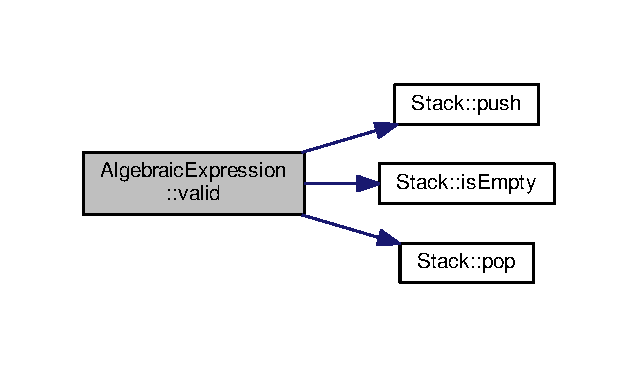
\includegraphics[width=306pt]{classAlgebraicExpression_aa3c08af8a2b4d67c356f3cf69b2f6bc6_cgraph}
\end{center}
\end{figure}




\subsection{Friends And Related Function Documentation}
\index{Algebraic\+Expression@{Algebraic\+Expression}!operator$>$$>$@{operator$>$$>$}}
\index{operator$>$$>$@{operator$>$$>$}!Algebraic\+Expression@{Algebraic\+Expression}}
\subsubsection[{\texorpdfstring{operator$>$$>$}{operator>>}}]{\setlength{\rightskip}{0pt plus 5cm}istream\& operator$>$$>$ (
\begin{DoxyParamCaption}
\item[{istream \&}]{ins, }
\item[{{\bf Algebraic\+Expression} \&}]{ae}
\end{DoxyParamCaption}
)\hspace{0.3cm}{\ttfamily [friend]}}\hypertarget{classAlgebraicExpression_af703364bc81e99767331bb9e915ef6ff}{}\label{classAlgebraicExpression_af703364bc81e99767331bb9e915ef6ff}

\begin{DoxyCode}
143 \{
144    ins >> ae.\hyperlink{classAlgebraicExpression_ac9a5d8af4bd13370e7f2cb66b0f1daa2}{infix}; \textcolor{comment}{//the only thing initially needed in an AlgebraicExpression is the infix
       expression                                                                                                     }
145 \}
\end{DoxyCode}


\subsection{Member Data Documentation}
\index{Algebraic\+Expression@{Algebraic\+Expression}!infix@{infix}}
\index{infix@{infix}!Algebraic\+Expression@{Algebraic\+Expression}}
\subsubsection[{\texorpdfstring{infix}{infix}}]{\setlength{\rightskip}{0pt plus 5cm}string Algebraic\+Expression\+::infix\hspace{0.3cm}{\ttfamily [private]}}\hypertarget{classAlgebraicExpression_ac9a5d8af4bd13370e7f2cb66b0f1daa2}{}\label{classAlgebraicExpression_ac9a5d8af4bd13370e7f2cb66b0f1daa2}
\index{Algebraic\+Expression@{Algebraic\+Expression}!operand\+Stack@{operand\+Stack}}
\index{operand\+Stack@{operand\+Stack}!Algebraic\+Expression@{Algebraic\+Expression}}
\subsubsection[{\texorpdfstring{operand\+Stack}{operandStack}}]{\setlength{\rightskip}{0pt plus 5cm}{\bf Stack}$<$int$>$ Algebraic\+Expression\+::operand\+Stack\hspace{0.3cm}{\ttfamily [private]}}\hypertarget{classAlgebraicExpression_a8f0ee1ac59e782a546a7de47e507b391}{}\label{classAlgebraicExpression_a8f0ee1ac59e782a546a7de47e507b391}
\index{Algebraic\+Expression@{Algebraic\+Expression}!operator\+Stack@{operator\+Stack}}
\index{operator\+Stack@{operator\+Stack}!Algebraic\+Expression@{Algebraic\+Expression}}
\subsubsection[{\texorpdfstring{operator\+Stack}{operatorStack}}]{\setlength{\rightskip}{0pt plus 5cm}{\bf Stack}$<$char$>$ Algebraic\+Expression\+::operator\+Stack\hspace{0.3cm}{\ttfamily [private]}}\hypertarget{classAlgebraicExpression_a863ef1cc73b9b3b49c199f1564cbcc2e}{}\label{classAlgebraicExpression_a863ef1cc73b9b3b49c199f1564cbcc2e}
\index{Algebraic\+Expression@{Algebraic\+Expression}!postfix@{postfix}}
\index{postfix@{postfix}!Algebraic\+Expression@{Algebraic\+Expression}}
\subsubsection[{\texorpdfstring{postfix}{postfix}}]{\setlength{\rightskip}{0pt plus 5cm}string Algebraic\+Expression\+::postfix\hspace{0.3cm}{\ttfamily [private]}}\hypertarget{classAlgebraicExpression_a0c9827f84bf13c0f0f4a096e72462a44}{}\label{classAlgebraicExpression_a0c9827f84bf13c0f0f4a096e72462a44}
\index{Algebraic\+Expression@{Algebraic\+Expression}!result@{result}}
\index{result@{result}!Algebraic\+Expression@{Algebraic\+Expression}}
\subsubsection[{\texorpdfstring{result}{result}}]{\setlength{\rightskip}{0pt plus 5cm}int Algebraic\+Expression\+::result\hspace{0.3cm}{\ttfamily [private]}}\hypertarget{classAlgebraicExpression_a13af7ae171ff8616e6ab013a9cee9d75}{}\label{classAlgebraicExpression_a13af7ae171ff8616e6ab013a9cee9d75}


The documentation for this class was generated from the following files\+:\begin{DoxyCompactItemize}
\item 
\hyperlink{AlgebraicExpression_8h}{Algebraic\+Expression.\+h}\item 
\hyperlink{AlgebraicExpression_8cpp}{Algebraic\+Expression.\+cpp}\end{DoxyCompactItemize}

\hypertarget{classStack}{}\section{Stack$<$ T $>$ Class Template Reference}
\label{classStack}\index{Stack$<$ T $>$@{Stack$<$ T $>$}}


{\ttfamily \#include $<$Stack.\+h$>$}

\subsection*{Public Member Functions}
\begin{DoxyCompactItemize}
\item 
\hyperlink{classStack_aefee698059467258bbd79045aca62a63}{Stack} ()
\item 
\hyperlink{classStack_aa16507e9c77cb9be516b0980b346b7ec}{Stack} (vector$<$ T $>$ v)
\item 
void \hyperlink{classStack_a2723aec5c7e2611b97fcffeb7709de33}{pop} ()
\item 
T \hyperlink{classStack_ad461f6de40c8672dbf743068f4515061}{top} ()
\item 
void \hyperlink{classStack_a3553a0aa2c9640c5266e4d8790863e2e}{push} (T t)
\item 
bool \hyperlink{classStack_ad0db0d9b249e871bb7504ed89a99d3a7}{is\+Empty} ()
\item 
T \hyperlink{classStack_adcb4774ac8aa94cbc19b461da9bdee3a}{peek} ()
\item 
int \hyperlink{classStack_a3091d98f798b1b3e69b644d5b778c428}{size} ()
\end{DoxyCompactItemize}
\subsection*{Private Attributes}
\begin{DoxyCompactItemize}
\item 
vector$<$ T $>$ \hyperlink{classStack_aaf0fda0673d6b2d1670600ebe3b82f39}{stack}
\end{DoxyCompactItemize}


\subsection{Constructor \& Destructor Documentation}
\index{Stack@{Stack}!Stack@{Stack}}
\index{Stack@{Stack}!Stack@{Stack}}
\subsubsection[{\texorpdfstring{Stack()}{Stack()}}]{\setlength{\rightskip}{0pt plus 5cm}template$<$class T$>$ {\bf Stack}$<$ T $>$\+::{\bf Stack} (
\begin{DoxyParamCaption}
{}
\end{DoxyParamCaption}
)\hspace{0.3cm}{\ttfamily [inline]}}\hypertarget{classStack_aefee698059467258bbd79045aca62a63}{}\label{classStack_aefee698059467258bbd79045aca62a63}

\begin{DoxyCode}
27 \{\} \textcolor{comment}{//default constructor                                                                                   
                                                                                            }
\end{DoxyCode}
\index{Stack@{Stack}!Stack@{Stack}}
\index{Stack@{Stack}!Stack@{Stack}}
\subsubsection[{\texorpdfstring{Stack(vector$<$ T $>$ v)}{Stack(vector< T > v)}}]{\setlength{\rightskip}{0pt plus 5cm}template$<$class T$>$ {\bf Stack}$<$ T $>$\+::{\bf Stack} (
\begin{DoxyParamCaption}
\item[{vector$<$ T $>$}]{v}
\end{DoxyParamCaption}
)}\hypertarget{classStack_aa16507e9c77cb9be516b0980b346b7ec}{}\label{classStack_aa16507e9c77cb9be516b0980b346b7ec}

\begin{DoxyCode}
39 \{
40    \textcolor{keywordflow}{for}(\textcolor{keywordtype}{int} k=0; k<v.size(); k++)
41       \hyperlink{classStack_aaf0fda0673d6b2d1670600ebe3b82f39}{stack}.push\_back(v[k]);
42 \}
\end{DoxyCode}


\subsection{Member Function Documentation}
\index{Stack@{Stack}!is\+Empty@{is\+Empty}}
\index{is\+Empty@{is\+Empty}!Stack@{Stack}}
\subsubsection[{\texorpdfstring{is\+Empty()}{isEmpty()}}]{\setlength{\rightskip}{0pt plus 5cm}template$<$class T $>$ bool {\bf Stack}$<$ T $>$\+::is\+Empty (
\begin{DoxyParamCaption}
{}
\end{DoxyParamCaption}
)}\hypertarget{classStack_ad0db0d9b249e871bb7504ed89a99d3a7}{}\label{classStack_ad0db0d9b249e871bb7504ed89a99d3a7}

\begin{DoxyCode}
70 \{
71    \textcolor{keywordtype}{bool} empty = \textcolor{keyword}{true};
72    \textcolor{keywordflow}{if}(\hyperlink{classStack_aaf0fda0673d6b2d1670600ebe3b82f39}{stack}.size() > 0)
73       empty = \textcolor{keyword}{false};
74    \textcolor{keywordflow}{return} empty;
75 \}
\end{DoxyCode}
\index{Stack@{Stack}!peek@{peek}}
\index{peek@{peek}!Stack@{Stack}}
\subsubsection[{\texorpdfstring{peek()}{peek()}}]{\setlength{\rightskip}{0pt plus 5cm}template$<$class T $>$ T {\bf Stack}$<$ T $>$\+::peek (
\begin{DoxyParamCaption}
{}
\end{DoxyParamCaption}
)}\hypertarget{classStack_adcb4774ac8aa94cbc19b461da9bdee3a}{}\label{classStack_adcb4774ac8aa94cbc19b461da9bdee3a}

\begin{DoxyCode}
79 \{
80    T t;
81    \textcolor{keywordflow}{if}(!\hyperlink{classStack_ad0db0d9b249e871bb7504ed89a99d3a7}{isEmpty}())
82       t = \hyperlink{classStack_aaf0fda0673d6b2d1670600ebe3b82f39}{stack}.back(); \textcolor{comment}{//access element                                                              
                                                                                                            }
83    \textcolor{keywordflow}{return} t;
84 \}
\end{DoxyCode}
\index{Stack@{Stack}!pop@{pop}}
\index{pop@{pop}!Stack@{Stack}}
\subsubsection[{\texorpdfstring{pop()}{pop()}}]{\setlength{\rightskip}{0pt plus 5cm}template$<$class T $>$ void {\bf Stack}$<$ T $>$\+::pop (
\begin{DoxyParamCaption}
{}
\end{DoxyParamCaption}
)}\hypertarget{classStack_a2723aec5c7e2611b97fcffeb7709de33}{}\label{classStack_a2723aec5c7e2611b97fcffeb7709de33}

\begin{DoxyCode}
46 \{
47    \textcolor{keywordflow}{if}(!\hyperlink{classStack_ad0db0d9b249e871bb7504ed89a99d3a7}{isEmpty}())
48       \hyperlink{classStack_aaf0fda0673d6b2d1670600ebe3b82f39}{stack}.pop\_back();
49 \}
\end{DoxyCode}
\index{Stack@{Stack}!push@{push}}
\index{push@{push}!Stack@{Stack}}
\subsubsection[{\texorpdfstring{push(\+T t)}{push(T t)}}]{\setlength{\rightskip}{0pt plus 5cm}template$<$class T$>$ void {\bf Stack}$<$ T $>$\+::push (
\begin{DoxyParamCaption}
\item[{T}]{t}
\end{DoxyParamCaption}
)}\hypertarget{classStack_a3553a0aa2c9640c5266e4d8790863e2e}{}\label{classStack_a3553a0aa2c9640c5266e4d8790863e2e}

\begin{DoxyCode}
64 \{
65    \hyperlink{classStack_aaf0fda0673d6b2d1670600ebe3b82f39}{stack}.push\_back(t);
66 \}
\end{DoxyCode}
\index{Stack@{Stack}!size@{size}}
\index{size@{size}!Stack@{Stack}}
\subsubsection[{\texorpdfstring{size()}{size()}}]{\setlength{\rightskip}{0pt plus 5cm}template$<$class T $>$ int {\bf Stack}$<$ T $>$\+::size (
\begin{DoxyParamCaption}
{}
\end{DoxyParamCaption}
)}\hypertarget{classStack_a3091d98f798b1b3e69b644d5b778c428}{}\label{classStack_a3091d98f798b1b3e69b644d5b778c428}

\begin{DoxyCode}
88 \{
89    \textcolor{keywordflow}{return} \hyperlink{classStack_aaf0fda0673d6b2d1670600ebe3b82f39}{stack}.size(); \textcolor{comment}{//size of vector                                                              
                                                                                                            }
90 \}
\end{DoxyCode}
\index{Stack@{Stack}!top@{top}}
\index{top@{top}!Stack@{Stack}}
\subsubsection[{\texorpdfstring{top()}{top()}}]{\setlength{\rightskip}{0pt plus 5cm}template$<$class T $>$ T {\bf Stack}$<$ T $>$\+::top (
\begin{DoxyParamCaption}
{}
\end{DoxyParamCaption}
)}\hypertarget{classStack_ad461f6de40c8672dbf743068f4515061}{}\label{classStack_ad461f6de40c8672dbf743068f4515061}

\begin{DoxyCode}
53 \{
54    T t;
55    \textcolor{keywordflow}{if}(!\hyperlink{classStack_ad0db0d9b249e871bb7504ed89a99d3a7}{isEmpty}())
56    \{
57       t = \hyperlink{classStack_aaf0fda0673d6b2d1670600ebe3b82f39}{stack}.back(); \textcolor{comment}{//access top element                                                          
                                                                                                            }
58       \hyperlink{classStack_aaf0fda0673d6b2d1670600ebe3b82f39}{stack}.pop\_back(); \textcolor{comment}{//descard top element                                                         
                                                                                                            }
59    \}
60 \}
\end{DoxyCode}


\subsection{Member Data Documentation}
\index{Stack@{Stack}!stack@{stack}}
\index{stack@{stack}!Stack@{Stack}}
\subsubsection[{\texorpdfstring{stack}{stack}}]{\setlength{\rightskip}{0pt plus 5cm}template$<$class T$>$ vector$<$T$>$ {\bf Stack}$<$ T $>$\+::stack\hspace{0.3cm}{\ttfamily [private]}}\hypertarget{classStack_aaf0fda0673d6b2d1670600ebe3b82f39}{}\label{classStack_aaf0fda0673d6b2d1670600ebe3b82f39}


The documentation for this class was generated from the following file\+:\begin{DoxyCompactItemize}
\item 
\hyperlink{Stack_8h}{Stack.\+h}\end{DoxyCompactItemize}

\chapter{File Documentation}
\hypertarget{AEmain_8cpp}{}\section{A\+Emain.\+cpp File Reference}
\label{AEmain_8cpp}\index{A\+Emain.\+cpp@{A\+Emain.\+cpp}}
{\ttfamily \#include \char`\"{}Algebraic\+Expression.\+h\char`\"{}}\\*
{\ttfamily \#include \char`\"{}Stack.\+h\char`\"{}}\\*
Include dependency graph for A\+Emain.\+cpp\+:
\nopagebreak
\begin{figure}[H]
\begin{center}
\leavevmode
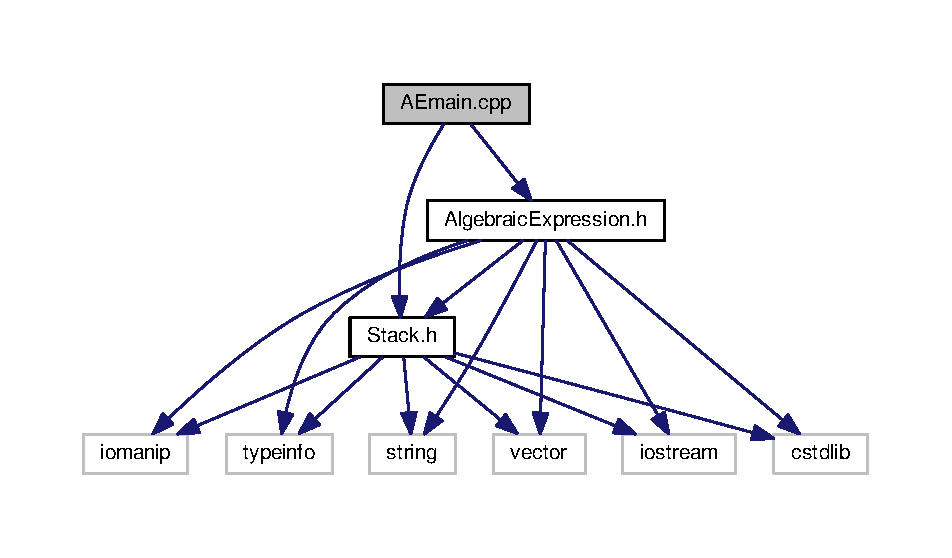
\includegraphics[width=350pt]{AEmain_8cpp__incl}
\end{center}
\end{figure}
\subsection*{Functions}
\begin{DoxyCompactItemize}
\item 
int \hyperlink{AEmain_8cpp_ae66f6b31b5ad750f1fe042a706a4e3d4}{main} ()
\end{DoxyCompactItemize}


\subsection{Function Documentation}
\index{A\+Emain.\+cpp@{A\+Emain.\+cpp}!main@{main}}
\index{main@{main}!A\+Emain.\+cpp@{A\+Emain.\+cpp}}
\subsubsection[{\texorpdfstring{main()}{main()}}]{\setlength{\rightskip}{0pt plus 5cm}int main (
\begin{DoxyParamCaption}
{}
\end{DoxyParamCaption}
)}\hypertarget{AEmain_8cpp_ae66f6b31b5ad750f1fe042a706a4e3d4}{}\label{AEmain_8cpp_ae66f6b31b5ad750f1fe042a706a4e3d4}

\begin{DoxyCode}
17 \{
18    \hyperlink{classAlgebraicExpression}{AlgebraicExpression}* aPtr;
19    \textcolor{keywordtype}{string} s;
20    cout << \textcolor{stringliteral}{"\(\backslash\)nEnter an equation or - to quit: "};
21    cin >> s;
22    \textcolor{keywordflow}{while}(s != \textcolor{stringliteral}{"-"})
23    \{
24       aPtr = \textcolor{keyword}{new} \hyperlink{classAlgebraicExpression}{AlgebraicExpression}(s);
25       \textcolor{keywordflow}{while}(!aPtr->\hyperlink{classAlgebraicExpression_aa3c08af8a2b4d67c356f3cf69b2f6bc6}{valid}())
26       \{
27          cout << \textcolor{stringliteral}{"\(\backslash\)nExpression is invalid! Please enter a new expression: "};
28          cin >> s;
29          aPtr = \textcolor{keyword}{new} \hyperlink{classAlgebraicExpression}{AlgebraicExpression}(s);
30       \}
31       aPtr->\hyperlink{classAlgebraicExpression_a0aeff15e3d0d529bd20a59f8d312a38d}{evaluateInfix}();
32       aPtr->\hyperlink{classAlgebraicExpression_ac0428ac1f1072f14e1391527baebd330}{evaluatePostfix}();
33       cout << aPtr->\hyperlink{classAlgebraicExpression_afcf555b573e6083a8395677bf056aef1}{getResult}() << endl;
34       cout << \textcolor{stringliteral}{"\(\backslash\)nEnter an equation or - to quit: "};
35       cin >> s;
36    \}
37    cout << endl;
38 
39    \textcolor{keywordflow}{return} 0;
40 \}
\end{DoxyCode}


Here is the call graph for this function\+:
\nopagebreak
\begin{figure}[H]
\begin{center}
\leavevmode
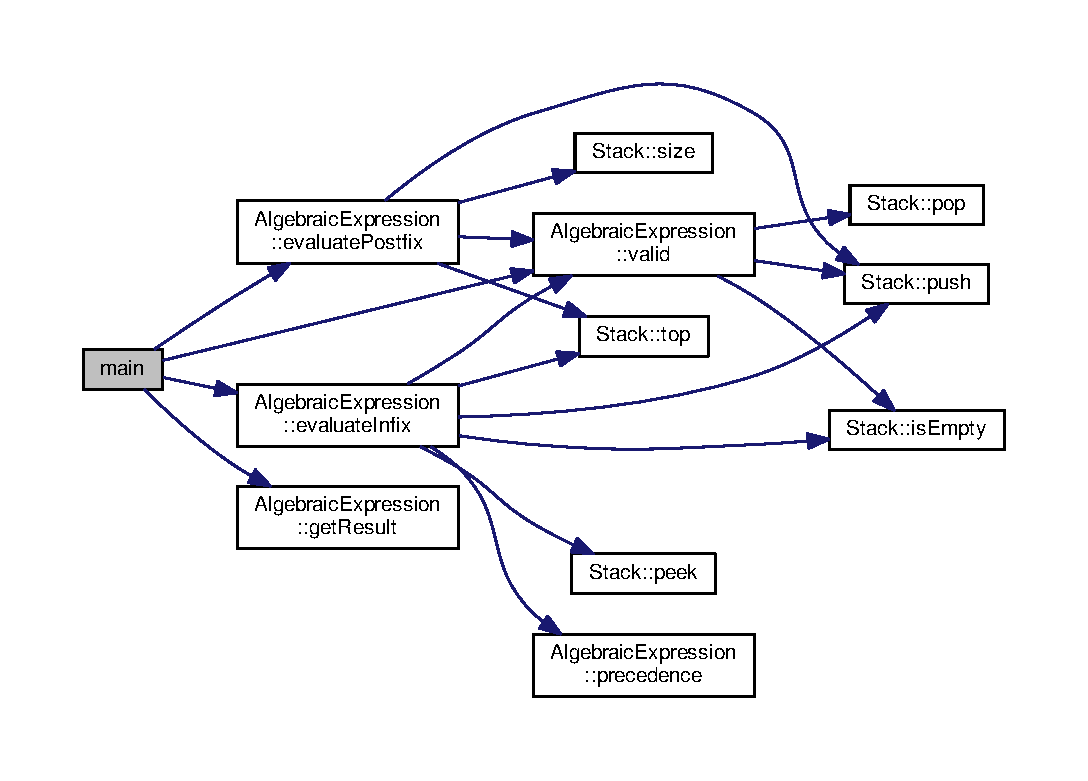
\includegraphics[width=350pt]{AEmain_8cpp_ae66f6b31b5ad750f1fe042a706a4e3d4_cgraph}
\end{center}
\end{figure}



\hypertarget{AlgebraicExpression_8cpp}{}\section{Algebraic\+Expression.\+cpp File Reference}
\label{AlgebraicExpression_8cpp}\index{Algebraic\+Expression.\+cpp@{Algebraic\+Expression.\+cpp}}
{\ttfamily \#include \char`\"{}Algebraic\+Expression.\+h\char`\"{}}\\*
Include dependency graph for Algebraic\+Expression.\+cpp\+:
\nopagebreak
\begin{figure}[H]
\begin{center}
\leavevmode
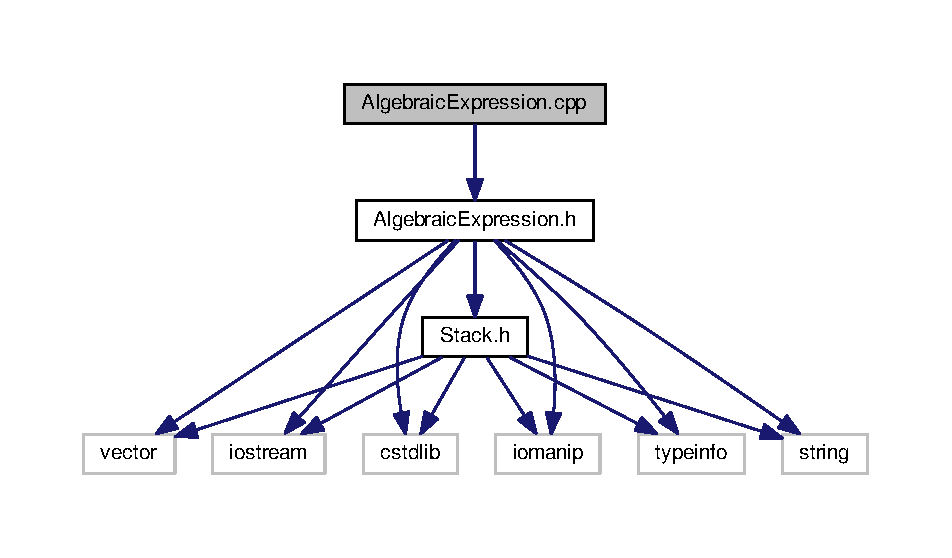
\includegraphics[width=350pt]{AlgebraicExpression_8cpp__incl}
\end{center}
\end{figure}
\subsection*{Functions}
\begin{DoxyCompactItemize}
\item 
istream \& \hyperlink{AlgebraicExpression_8cpp_af703364bc81e99767331bb9e915ef6ff}{operator$>$$>$} (istream \&ins, \hyperlink{classAlgebraicExpression}{Algebraic\+Expression} \&ae)
\end{DoxyCompactItemize}


\subsection{Function Documentation}
\index{Algebraic\+Expression.\+cpp@{Algebraic\+Expression.\+cpp}!operator$>$$>$@{operator$>$$>$}}
\index{operator$>$$>$@{operator$>$$>$}!Algebraic\+Expression.\+cpp@{Algebraic\+Expression.\+cpp}}
\subsubsection[{\texorpdfstring{operator$>$$>$(istream \&ins, Algebraic\+Expression \&ae)}{operator>>(istream &ins, AlgebraicExpression &ae)}}]{\setlength{\rightskip}{0pt plus 5cm}istream\& operator$>$$>$ (
\begin{DoxyParamCaption}
\item[{istream \&}]{ins, }
\item[{{\bf Algebraic\+Expression} \&}]{ae}
\end{DoxyParamCaption}
)}\hypertarget{AlgebraicExpression_8cpp_af703364bc81e99767331bb9e915ef6ff}{}\label{AlgebraicExpression_8cpp_af703364bc81e99767331bb9e915ef6ff}

\begin{DoxyCode}
143 \{
144    ins >> ae.\hyperlink{classAlgebraicExpression_ac9a5d8af4bd13370e7f2cb66b0f1daa2}{infix}; \textcolor{comment}{//the only thing initially needed in an AlgebraicExpression is the infix
       expression                                                                                                     }
145 \}
\end{DoxyCode}

\hypertarget{AlgebraicExpression_8h}{}\section{Algebraic\+Expression.\+h File Reference}
\label{AlgebraicExpression_8h}\index{Algebraic\+Expression.\+h@{Algebraic\+Expression.\+h}}
{\ttfamily \#include \char`\"{}Stack.\+h\char`\"{}}\\*
{\ttfamily \#include $<$iostream$>$}\\*
{\ttfamily \#include $<$string$>$}\\*
{\ttfamily \#include $<$vector$>$}\\*
{\ttfamily \#include $<$cstdlib$>$}\\*
{\ttfamily \#include $<$iomanip$>$}\\*
{\ttfamily \#include $<$typeinfo$>$}\\*
Include dependency graph for Algebraic\+Expression.\+h\+:
\nopagebreak
\begin{figure}[H]
\begin{center}
\leavevmode
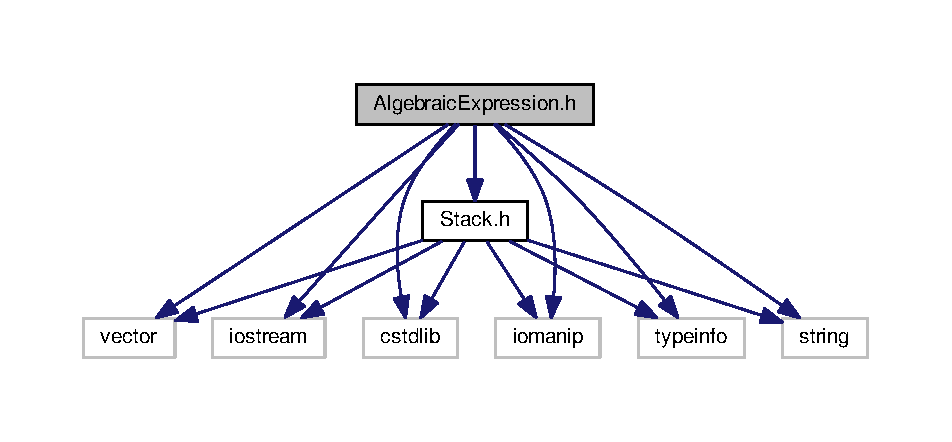
\includegraphics[width=350pt]{AlgebraicExpression_8h__incl}
\end{center}
\end{figure}
This graph shows which files directly or indirectly include this file\+:
\nopagebreak
\begin{figure}[H]
\begin{center}
\leavevmode
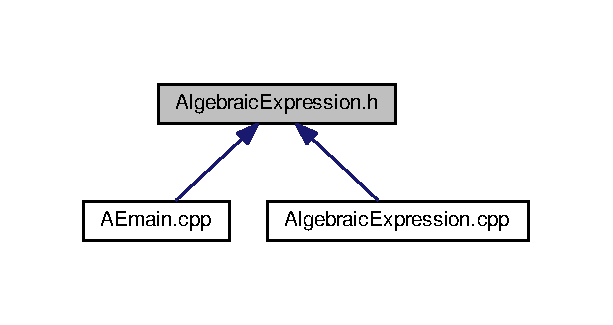
\includegraphics[width=294pt]{AlgebraicExpression_8h__dep__incl}
\end{center}
\end{figure}
\subsection*{Classes}
\begin{DoxyCompactItemize}
\item 
class \hyperlink{classAlgebraicExpression}{Algebraic\+Expression}
\end{DoxyCompactItemize}

\hypertarget{Stack_8h}{}\section{Stack.\+h File Reference}
\label{Stack_8h}\index{Stack.\+h@{Stack.\+h}}
{\ttfamily \#include $<$vector$>$}\\*
{\ttfamily \#include $<$iostream$>$}\\*
{\ttfamily \#include $<$cstdlib$>$}\\*
{\ttfamily \#include $<$iomanip$>$}\\*
{\ttfamily \#include $<$typeinfo$>$}\\*
{\ttfamily \#include $<$string$>$}\\*
Include dependency graph for Stack.\+h\+:
\nopagebreak
\begin{figure}[H]
\begin{center}
\leavevmode
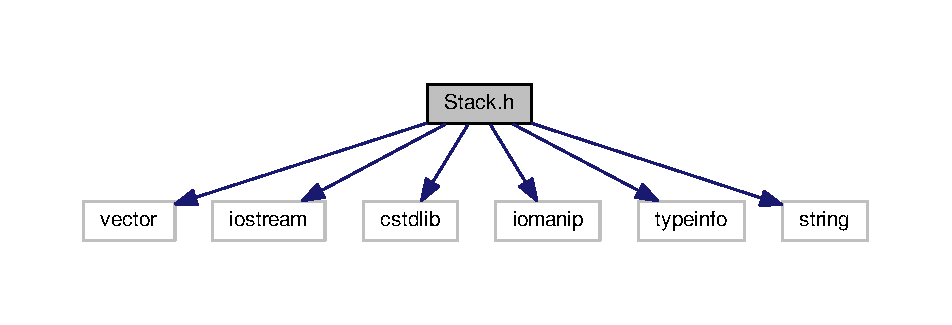
\includegraphics[width=350pt]{Stack_8h__incl}
\end{center}
\end{figure}
This graph shows which files directly or indirectly include this file\+:
\nopagebreak
\begin{figure}[H]
\begin{center}
\leavevmode
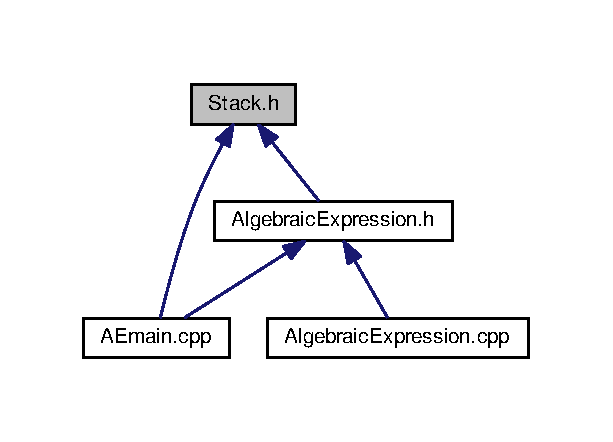
\includegraphics[width=294pt]{Stack_8h__dep__incl}
\end{center}
\end{figure}
\subsection*{Classes}
\begin{DoxyCompactItemize}
\item 
class \hyperlink{classStack}{Stack$<$ T $>$}
\end{DoxyCompactItemize}

%--- End generated contents ---

% Index
\backmatter
\newpage
\phantomsection
\clearemptydoublepage
\addcontentsline{toc}{chapter}{Index}
\printindex

\end{document}
